\subsubsection{Electronic Devices and Nanophotonics}
\index{Knipp, Dietmar}

\paragraph{Research Team}
Dietmar Knipp (Professor), Amare Benor, Kah-Yoong Chan, Christian Haase (external PhD
student)  (PhD Student), Rahul Dewan (MSc student), Zhelio Andreev (MSc student)\\

Research of the Electronic Devices and Nanophotonics group is focused on nano and optical technologies
 and their applications in information technology and photovoltaics. The major goal is to develop the next generation of electronic and photonic devices bridging from the micro to the nanoscale.

\paragraph{Highlights}

Organic materials provide a variety of interesting and new properties, which facilitate
the realization of electronic devices like Thin-Film-Transistors (TFT), flexible displays
and wireless information tags (RFID tags). Organic TFTs provide two major advantages over
'classical' TFTs based on amorphous or polycrystalline silicon. They can be fabricated at
very low temperatures ($<100^\circ$ C) and, potentially, at significantly lower cost. The
prospect of electronics at relatively low cost has stimulated a lot of R\&D on displays,
imagers for medical, industrial, and consumer applications.  A cross section of a thin
film transistor (TFT) is shown in figure~\ref{fig:profknipp} (bottom). Due to the low
fabrication temperatures all layers of the transistor are realized on neutral substrates
like glass or plastic foils. The operating principle of a thin film transistor is
comparable to Metal-Oxide-Semiconductor Field-Effect-Transistors (MOSFET), which are used
in microeletronics. In order to realize Thin Film Transistors with high charge carrier
mobility and high stability the organic films have to be highly order. The packing of a
highly ordered pentacene film is shown in the figure~\ref{fig:profknipp} (top).


\begin{figure}[ht]
  \begin{center}
    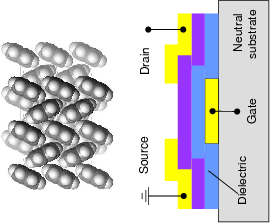
\includegraphics[width=\hsize,angle=-90]{Knipp/profknipp-fignano.png}
    \mycaption{Cross section of a thin film transistor (bottom) and packing of a highly
      order organic (pentacene) film (top)}\label{fig:profknipp}
   \end{center}
\end{figure}


Disorder of the pentacene molecules lead to a significant drop of the charge carrier
mobility. Further aspects have to be taken into account when realizing organic
transistors. In particular the influence of impurities on the device operation and the
device stability is still under investigation. The device behavior was studying by
electrical in-situ and ex-situ measurements (together with the research group of
Prof. V. Wagner) and numerical simulations using a density of states model (together with
Dr. A. V\"olkel, Palo Alto Research Center). The input parameters for the electrical
simulations can be determined by using first-principles pseudopotential density functional
calculations (Dr. J. Northrup, Palo Alto Research Center).  In terms of the application
the electronic device and nanophotonics group is working together with the Institute for
Microsensors and Actuators (IMSAS) at the University Bremen. Both groups are working on
the development of a compact micro projector system. The IMSAS has developed an optical
projection elements using state of the art MEMS (Micro-Electro-Mechanical-Systems) and
Micro-System-Technologies. The optical projection element (Fabry-Perot-resonator) acts as
an optical switch, which can be controlled by an applied bias voltage. The projector
elements are controlled by thin film transistors, which are integrated together with the
projector elements.  In summary, research on organic electronics facilities the
realization of a broad range of electronic devices like radio frequency identification
tags, displays and smart cards. The electronic device group is working on aspects ranging
from material science to applications.



\paragraph{Collaborations}
\begin{enumerate}
\item {\sl International University Bremen} \\ Prof. Veit Wagner \\ Organic Electronics
 \\ Prof. Werner Bergholz \\ Photovoltaics and Microelectronics
%\end{enumerate}
\item {\sl University Bremen} \\ Prof. Wolfgang Benecke \\ Microsystems Technology
\item {\sl Research Center J\"ulich} \\ Dr. Helmut Stiebig \\ Nanocrystalline Thin Film
  Transistors and Optics in nanostructured media
\item {\sl Bendit Innovative Interfaces} \\ J. Huyer \\ Solar Cells for mobile
  applications
\item {\sl Palo Alto Research Center} \\ Dr. R.A. Street, A.R. V\"olkel. Dr. J. Northrup
  \\ Organic electronics and modelling
\item {\sl Stanford University} \\ Prof. A. Salleo \\ Organic electronics

\end{enumerate}


\paragraph{Other Support Grants}
% list the running grants in 2006, if none have been received, please delete this
% subsection.
\begin{enumerate}
\item Funded by BMBF, \emph{Embedded Microsystems Bremen (EMB)}
\item Funded by Forschungszentrum J\"ulich, \emph{Funktionale Kontaktschichen}
\end{enumerate}


\paragraph{Awards, Prizes}
% list the grants you have received in 2005, if none have been received, please delete this
% subsection.
\begin{enumerate}
\item Ernst A.C. Lange Award together with Prof. W. Benecke from the Institute for
  Microsensors, -actuators, and -systems (University Bremen)
\end{enumerate}

\paragraph{Patents}
\begin{enumerate}
\item H. Stiebig, D. Knipp, J. F\"alsch, Three-color sensor with a pin or nip series of
  layers, Japan, Patent number: Hei-9-535750;
\item D. Knipp, Optical sensor and integrated photonic crystal and method for producing
  the optical sensor, submitted to German patent office.
\end{enumerate}

\nocite{Knipp1, Knipp2, Knipp3, Knipp4, Knipp5, Knipp6, Knipp7, Knipp8, Knipp9,
Knipp10, Knipp11}
